\chapter{Introduction}\label{chap:Introduction}

Satellites are no longer the privilege of just a handful of economic powerhouses such as nations or mega companies. There are currently 1738 active satellites orbiting Earth, 129 of it is categorized as having civil uses, created mostly for educational purposes \cite{SatSummary}. The ongoing AAUSAT project at Aalborg University is part of this educational effort. AAUSATs are mostly student built low-cost picosatellites, 5 of them already in orbit, the next one is currently in development \cite{aausatsite}. 
\nomenclature[TP]{\textbf{Picosatellite}}{Picosatellites are small satellites with mass between 0.1 and 1 kg.}
 The mission goal of each of them include taking pictures of Earth and celestial objects and downlink them, or even tracking objects on Earth's surface. These require precise attitude control of the satellite. 

Satellite attitude control differs fundamentally from the attitude control of earthbound objects, and is more challenging, as there is no direct mechanical connection available to other objects. Thus attitude control can be achieved using different interactions, such as transferring angular momentum between components of the satellite, utilizing the magnetic field of Earth or solar sails, or in some cases rocket propellants.

 While the satellites themselves can be chosen to be engineered relatively cheaply, there is no way of avoiding the high cost of putting the satellite into orbit. Many efforts were made recently to reduce this cost.  Since the cost is highly dependent on the weight of the satellite, by minimizing the weight, a lot of money can be saved. The per kilogram cost of putting an object to Low Earth Orbit (LEO) in the case of Falcon Heavy, 1655 USD \cite{spaceX}, however this price only applies for 54400 kg payload. There are rockets missions with the purpose of putting several satellites into orbit, thus reducing the cost for individual satellites. The sizing unit of the satellites involved in such missions is standardized. One unit is $10\times10\times10$ cm and 1 kg. AAU CUBESAT fits into one unit, thus costing 49000 USD to put in orbit \cite{AAUSATpres}. 
% Future AAUSATs might be put into orbit with Falcon 9 rocket. The per kilogram cost in low earth orbit SpaceX launch is less than $3000\$$ \cite{spaceX}, but the actual price for an individual satellite would be higher.
 
 The weight constraint had to be taken into account when designing each component of the satellite. For the attitude control system it means that using propellants excessively is not an option. To make quick attitude control possible, reaction wheels are used as actuators, supported by magnetorquers for desaturation. 
   
 Since putting satellites into orbit is quite costly, a lot of effort is made to prevent system failures. It is imperative to design the satellite in such a way that a fault in one of the modules does not lead to mission failure. The satellite is designed to withstand extreme temperature changes, large accelerations during launch etc. Every part is made to last as long as possible. Attitude estimation schemes are outside the scope of the thesis. In order to be able to handle faults in actuators, a fault-tolerant control scheme is implemented.  This thesis explores several fault detection and fault handling schemes involved in fault tolerant attitude control.
 
 \nomenclature[A]{\textbf{AAUSAT}}{The name of the satellites developed at Aalborg University} 
 
 
 \begin{figure}%[h!]
 	\centering 
 	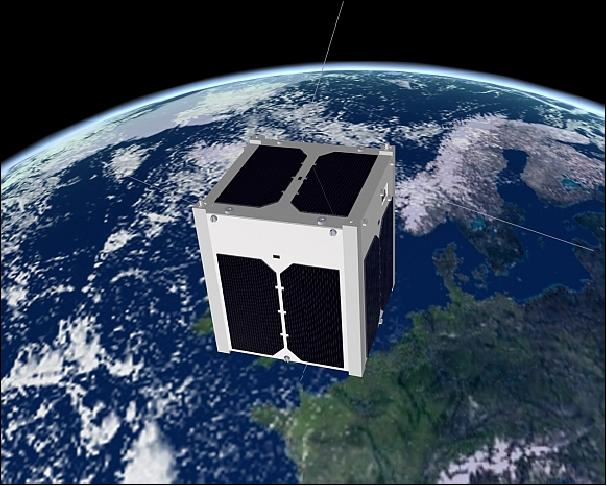
\includegraphics[width=80mm]{figures/aausatInSpace.jpg}	
 	\caption{AAUSAT on Duty. An Illustration. \cite{imref}}
 	\label{fig:aauinspace}
 \end{figure}

 
 \nomenclature[TP]{\textbf{Precession}}{A rotating body can experience a change in the orientation around the rotational axis.} 
 

\section{Problem statement}
The objective of the present thesis is to implement a fault-tolerant attitude control scheme for a pico-satellite equipped with magnetorquers and reaction wheels. The fault tolerant control scheme isolates actuator faults.

%Developing a solution for the case of fault detection and isolation that might occur in an actuator of a pico-satellite by design and simulation of a fault-tolerant attitude control scheme for a pico-satellite which is supplied with magnetorquers and reaction wheels will be the objective of this thesis.

\section{Use-case}\label{sec:useCase}
To further expand the problem statement stated above, a use case is conceived. In order to achieve the mission task, the use case is constructed for proving the system requirements.

The mission of AAUSAT-3 is used as a reference for establishing the use-case. One of the tasks of the pico-satellite is to track ships in arctic regions. This steams from the desire of the Danish Maritime Safety Administration \nomenclature[AD]{\textbf{DaMSA}}{Danish Maritime Safety Administration}(DaMSA) to improve naval safety by monitoring the ships. The test area would be around Greenland, where monitoring is lacking. % http://www.space.aau.dk/aausat3/index.php?n=Main.AAUSAT3MissionDescription


In order to achieve this objective, a Low Earth Orbit  \nomenclature[AL]{\textbf{LEO}}{Low Earth Orbit}  satellite is deployed and Automatic Identification System \nomenclature[AA]{\textbf{AIS}}{Automatic Identification System}(AIS) signals are used for exchanging information with a ground station. As secondary mission the satellite has to gather pictures of the Arctic regions.

If the requirement for the satellite is tracking objects on Earth, the tracking torque demand can be calculated using knowledge about satellite altitude, orbit shape and the corresponding satellite speed, and satellite moment of inertia. For a circular orbit at 600 km altitude, the satellite speed would be $7.56 km/s$  according to \cite{satSpeed}. Appendix \ref{chap:D} presents the graphs used in deriving the torque demand for Earth station pointing. A maximum torque of ${2.388 \times 10^{-7} Nm}$ was calculated, which acts as a requirement for the actuators torque output.